\apendice{Documentación de usuario}

\section{Introducción}

La documentación de usuario tiene como finalidad presentar una guía de requisitos necesarios para el correcto funcionamiento de la aplicación, un manual de instalación guiado paso a paso y la presentación de las opciones de interacción disponibles a través de la aplicación web para la obtención de resultados.

\section{Requisitos de usuarios}

Los requisitos de usuario sugieren una serie especificaciones hardware y software del equipo anfitrión de la aplicación de modo que el proyecto cumpla con los requisitos funcionales y no funcionales. Estas características son las siguientes:

\begin{itemize} \setlength\itemsep{0.2em}
    \item Sistema operativo Windows 10 o Ubuntu 20.04 o superior.
    \item 6GB de memoria RAM.
    \item 30GB de espacio libre en disco.
    \item Conexión a Internet estable.
    \item Navegador web: Google Chrome 96, Microsoft Edge 96, o Mozilla Firefox 94 o superior.
\end{itemize}

\section{Instalación}

En el siguiente apartado se presentan las instrucciones a través de las cuales establecer un entorno de desarrollo que disponga del código fuente, utilidades, complementos y ejecutables requeridos para la puesta en marcha del proyecto. 

\subsection{Prerrequisitos}
El código fuente del proyecto se ha implementado haciendo uso de los lenguajes de programación \textbf{Python} y \textbf{JavaScript}. En el caso de Python este se requiere para las implementaciones llevadas a cabo en el apartado del front-end. El uso de JavaScript se debe al desarrollo de la aplicación web, implementada sobre el entorno de ejecución \textbf{NodeJS}. A continuación se incluyen las versiones requeridas por la aplicación para asegurar su correcto funcionamiento:
\begin{itemize}
    \item \textbf{Python 3.9.6} o superior.
    \item \textbf{NodeJS 14.17.4} o superior.
    \item \textbf{Docker 20.10.12} o superior.
    \item \textbf{Docker Compose 1.29.2} o superior.
\end{itemize}

\subsection{Obtención el proyecto}

El proyecto se encuentra alojado en un repositorio de GitHub de acceso libre. Para proceder con la obtención de una copia local de los ficheros se recurrirá a un software de control de versiones que ofrezcan soporte a repositorios de GitHub como \textbf{Git} o \textbf{GitHub Desktop}. También es posible la descarga directa de los ficheros a través de la dirección de GitHub en la cual se encuentra alojado el repositorio. La dirección de acceso al repositorio es la siguiente:

\vspace{0.5cm}
\centerline{\texttt{\url{https://github.com/MrpYA45/github-text-mining-tfg}}}
\vspace{0.4cm}

En caso de que se haya decidido escoger el popular software de control de versiones Git el comando requerido para la obtención de los archivos es el siguiente:

\vspace{0.5cm}
\centerline{\texttt{git clone https://github.com/MrpYA45/github-text-mining-tfg}}
\vspace{0.4cm}

\begin{figure}[!ht]
	\centering
    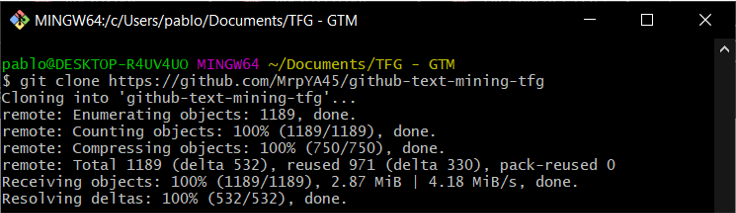
\includegraphics[width=\textwidth]{img/git_gtm.png}
	\caption{Obtención del repositorio mediante Git.}
	\label{fig:git_gtm_mu}
\end{figure}

\subsection{Instalación de las dependencias de la aplicación web}
A continuación, se procederá con la instalación de las dependencias de la aplicación web. Esta se encuentra construida sobre el entorno de ejecución NodeJS basado en JavaScript. La aplicación web también ha sido desarrollada haciendo uso de módulos que simplifican la programación de ciertos aspectos de la web.

Para proceder a la instalación de estas dependencias se deberá situar la terminal en la carpeta \texttt{src/webapp}. El fichero \texttt{package.json} es el encargado de almacenar el listado con las dependencias necesarias para poder proceder con la instalación, así como los \textit{scripts} que permiten lanzar la aplicación. Para proceder con la instalación de los ficheros necesarios se deberá recurrir al siguiente comando:

\vspace{0.5cm}
\centerline{\textbf{Windows/MacOS/Linux: } \texttt{npm install}}
\vspace{0.4cm}

\subsection{Lanzamiento de los servicios del back-end}

El lanzamiento de los servicios del back-end se realizará por medio del uso de las herramientas \textbf{Docker} y \textbf{Docker Compose}, para las cuales se ha diseñado una configuración que permite mantener cada uno de los servicios y la base de datos en contenedores independientes.

El primer paso consistirá en la obtención de las imágenes que se ejecutarán en el interior de los contenedores. Para ello, situándonos en la directorio raíz del proyecto, se deberá ejecutar el comando de construcción que se incluye a continuación. Se ha de tener en cuenta que la primera ejecución del comando requiere de la descarga de numerosos archivos pesados, por ello por lo que el proceso puede alargarse durante varios minutos.

\vspace{0.5cm}
\centerline{\textbf{Windows/MacOS/Linux:}}
\centerline{\texttt{docker-compose -f docker/config/docker-compose.yml build}}
\vspace{0.4cm}

Una vez se ha completado el proceso de generación de las imágenes se deberá proseguir con el levantamiento de los contenedores que contendrán dichas imágenes. En una primera instancia este proceso requiere de un extenso tiempo de espera durante el cual se procede a la descarga e instalación de las dependencias requeridas por los servicios en el interior de los propios contenedores.

\vspace{0.5cm}
\centerline{\textbf{Windows/MacOS/Linux:}}
\centerline{\texttt{docker-compose -f docker/config/docker-compose.yml up}}
\vspace{0.4cm}

El servicio con un mayor tiempo de despliegue inicial resulta ser el servicio de procesamiento denominado \textit{gtmprocessing}, el cual puede llegar a requerir de entre 10 y 15 minutos en su arranque. Ante la pobre vivacidad que se presenta en el proceso de obtención de los modelos se recomienda realizar comprobaciones periódicas a través del siguiente comando.

\vspace{0.5cm}
\centerline{\textbf{Windows/MacOS/Linux: } \texttt{docker logs gtmprocessing -t}}
\vspace{0.4cm}

Esta orden permite obtener un visualizar la actividad que se está produciendo en el interior del contenedor. A través de esta salida se podrá comprobar el estado de la descarga de los modelos.

\subsubsection{Configuración inicial de los servicios}

Una vez finalizado el proceso de configuración inicial se deberá verificar que se han generado correctamente los ficheros de configuración. Estos ficheros se encuentran en el interior de cada uno de los servicios en la ruta \texttt{/src/backend/\%service\_name\%/config}.

Verificada la existencia de estos ficheros se deberán detener los contenedores para poder proceder a su pertinente configuración.

\vspace{0.5cm}
\centerline{\textbf{Windows/MacOS/Linux:}}
\centerline{\texttt{docker-compose -f docker/config/docker-compose.yml stop}}
\vspace{0.4cm}

Cada servicio dispone de una carpeta \textit{gtmcore} en su configuración que permite alterar los parámetros de conexión con la base de datos. Por defecto, estos ficheros se generan con una configuración básica de acuerdo con la configuración de la base de datos establecida en el fichero de variables de entorno de Docker localizado en la siguiente ruta \texttt{docker/services/.env}. Se recomienda encarecidamente modificar estos valores en caso de lanzar la aplicación en algún entorno de producción.

Finalmente, el servicio de extracción dispone de una segunda carpeta de configuración denominada \textit{gtmprocessing}. En su interior se encuentra un fichero de configuración que se requiere completar para lograr la extracción de la información de los repositorios. Este fichero solicita un token de acceso personal de GitHub.

Una vez se haya completado la configuración de los servicios se deberá volver a levantar los contenedores con el comando señalado anteriormente. En el momento en que los servicios se encuentren completamente desplegados será posible acceder a la API REST de la aplicación por medio de consultas a la dirección \url{http://localhost:6060/}.

\subsubsection{Obtención de un token de acceso personal de GitHub}

La obtención de un token de acceso personal de GitHub requiere de encontrarnos registrados en la plataforma. Una vez en ella se puede solicitar el token desde el apartado de \textit{Settings}, \textit{Developer Settings}, y seleccionar el apartado \href{https://github.com/settings/tokens}{\textit{Personal Access Tokens}}.

La generación de un token requiere del establecimiento de un periodo de caducidad y de la selección de una serie de permisos básicos para poder realizar ciertas acciones. El uso básico de las peticiones que se realizan por parte de la aplicación implica que solo se requiere del permiso de acceso a repositorios públicos (véase \autoref{fig:gen_github_access_tokens_mu}).

\begin{figure}[!ht]
	\centering
    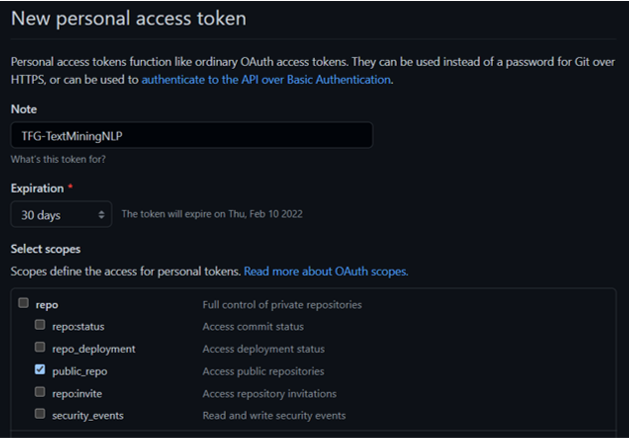
\includegraphics[width=\textwidth]{img/gen_github_access_tokens.png}
	\caption{Generación del Token de Acceso Personal en GitHub.}
	\label{fig:gen_github_access_tokens_mu}
\end{figure}

\subsection{Lanzamiento de la aplicación web mediante NodeJS}

El lanzamiento de aplicación web solamente requiere de la situación de la terminal en la ruta donde se localiza los ficheros de la aplicación web (\texttt{src/webapp}) y la introducción del siguiente comando. 

\vspace{0.5cm}
\centerline{\textbf{Windows/MacOS/Linux: } \texttt{npm start gtm-webapp}}
\vspace{0.4cm}

Tras su ejecución se producirá el despliegue de la aplicación en un servidor de NodeJS y la apertura automática de una ventana en el navegador web presentando al usuario la web. En caso de que esto no suceda por algún motivo desconocido, la aplicación web se encuentra accesible desde la siguiente dirección \url{http://localhost:3000/}.

\section{Manual del usuario}

El manual de usuario tiene como finalidad ilustrar el uso de la interfaz web de la aplicación.

\subsection{Selección y obtención de repositorios}

El primer paso requerido para explotar las funcionalidades de la aplicación consiste en incorporar los datos de los repositorios a la aplicación. Para ello, el usuario deberá hacer clic sobre el apartado ''\textbf{Repositorios}'' de la web. En esta sección se podrá observar un listado de los repositorios disponibles debido a que hayan sido cargados previamente por el usuario, así como un formulario en una sección inferior que permite incorporar nuevos repositorios al sistema (véase \autoref{fig:webapp_list_and_get_repo}).

\begin{figure}[!ht]
	\centering
    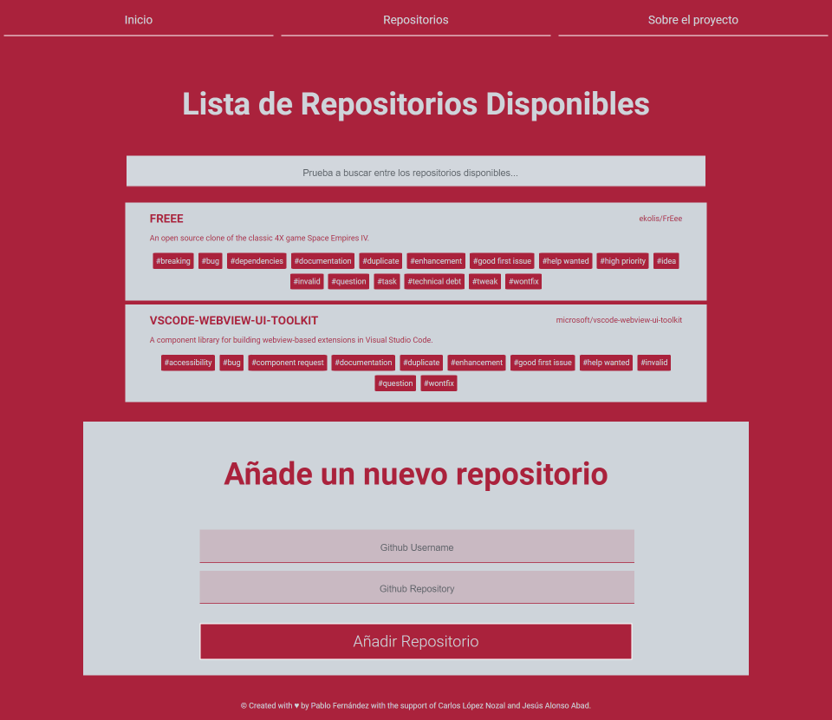
\includegraphics[width=\textwidth]{img/webapp_list_and_get_repo.png}
	\caption{Sección ''\textbf{Repositorios}'' de la aplicación web.}
	\label{fig:webapp_list_and_get_repo}
\end{figure}

El procedimiento para incorporar nuevos repositorios requiere de la introducción de una combinación válida de usuario y repositorio de \textbf{GitHub}. Una vez se introduzcan los datos y se pulse sobre el botón de añadir repositorio se encolará dicha petición, siempre y cuando el \textit{back-end} de la aplicación se encuentre debidamente desplegado. El usuario recibirá una notificación indicando si la petición ha podido ser encolada satisfactoriamente o no.

Tenga en cuenta que la introducción de una combinación incorrecta no producirá un error debido a que la notificación solo indica la recepción del trabajo por parte del \textit{back-end}, no su resultado. En caso de que esta combinación resulte incorrecta la tarea quedará rechazada por el \textit{backend} y el proceso no continuará.

Una vez completado el formulario el usuario será redirigido a una nueva pestaña mientras se produce la extracción de los datos. En caso de que se le notifique que el proceso no ha podido continuar, regrese a la pestaña anterior. La detección de una combinación incorrecta no dispone de indicativos visuales, si detecta largos tiempos de espera incoherentes con el tamaño de su repositorio (calculado en función del número de incidencias y sus comentarios), por favor regrese a la sección de Repositorios.

\subsection{Lanzar experimentos}

Una vez la descarga de la información del repositorio se haya completado satisfactoriamente el usuario deberá ser capaz de poder visualizar a una nueva sección de la aplicación. Esta vista presenta una introducción con los datos principales del repositorio y una serie de formularios de acuerdo con los experimentos disponibles.

\subsubsection{Zero-Shot Classification}

Este formulario permite al usuario la aplicación de un modelo de clasificación Zero-Shot sobre las incidencias del repositorio (véase \autoref{fig:webapp_zsc_form}). El objetivo de este experimento consiste en, partiendo de una incidencia y de una serie de etiquetas, asignar una puntuación entre 0 y 1 a cada etiqueta de acuerdo con la probabilidad de que su temática se corresponda con la temática de la incidencia. Por defecto, las únicas etiquetas utilizadas son aquellas definidas por el repositorio para su clasificación manual.

\begin{figure}[!ht]
	\centering
    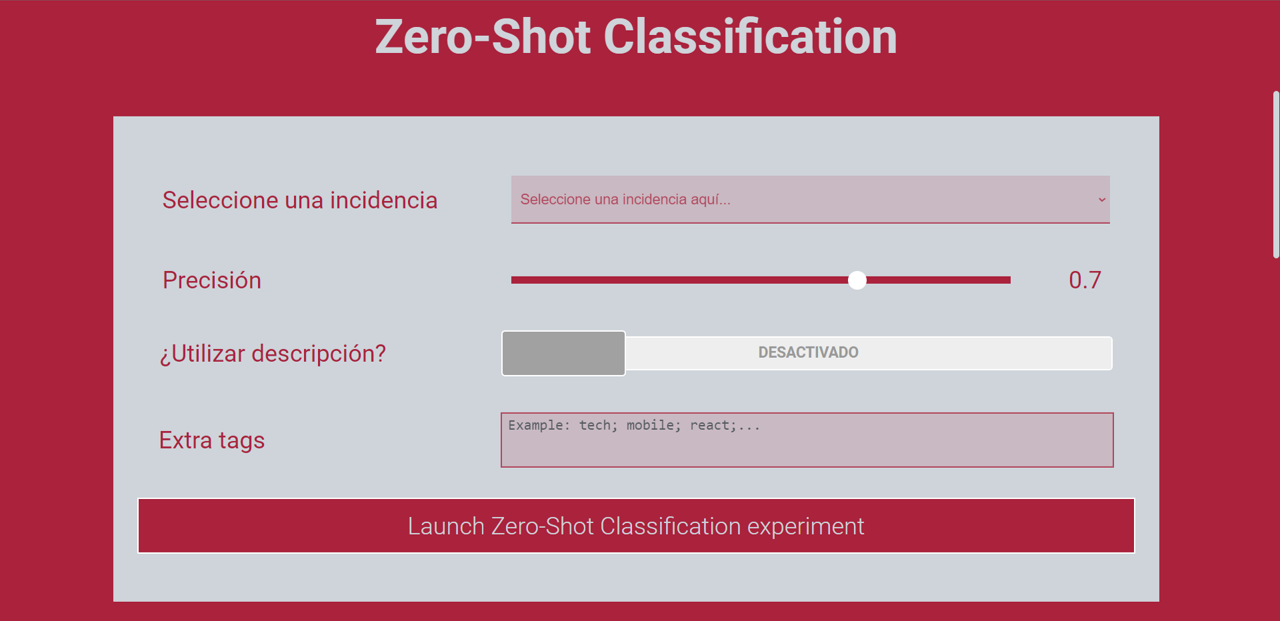
\includegraphics[width=\textwidth]{img/webapp_zsc_form.png}
	\caption{Formulario de lanzamiento de experimento de Zero-Shot Classification.}
	\label{fig:webapp_zsc_form}
\end{figure}

Los parámetros disponibles son los siguientes: 

\begin{itemize} \setlength\itemsep{0.2em}
    \item \textbf{Selección de incidencia}. Este parámetro permite seleccionar mediante un desplegable las incidencias del repositorio de acuerdo con su título. Es posible que observe más incidencias que las disponibles en su sección homónima en su repositorio de GitHub. Esto se debe a que GitHub trata internamente las ''\textit{pull request}'', o solicitudes de incorporación de cambios, como una extensión vitaminada de las incidencias. Como estas también incluyen un apartado de discusión, también es posible trabajar con ellas durante los experimentos.
    \item \textbf{Precisión}. El \textit{slider} de la precisión permite al usuario indicar un umbral a partir del cual las etiquetas que se encuentren por debajo de este no serán mostradas como resultado válido.
    \item \textbf{Utilizar descripción}. Este parámetro permite otorgar un mayor contexto al modelo incluyendo la información correspondiente con la descripción de la incidencia en la realización de sus operaciones. Por defecto el modelo sólo utiliza la información deducida a partir de su título.
    \item \textbf{Etiquetas extra}. Este parámetro permite añadir etiquetas fuera de aquellas declaradas por el propio repositorio en GitHub. Las etiquetas deberán introducirse en el cuadro de texto separadas haciendo uso del carácter punto y coma entre ellas.
\end{itemize}

Los resultados del experimento se presentan en forma de de un gráfico circular que contiene aquellas etiquetas que sobrepasan el umbral establecido en los parámetros. El tamaño de las secciones representa la probabilidad de pertenencia a cada una de las temáticas propuestas (véase \autoref{fig:webapp_zsc_output}).

\begin{figure}[!ht]
	\centering
    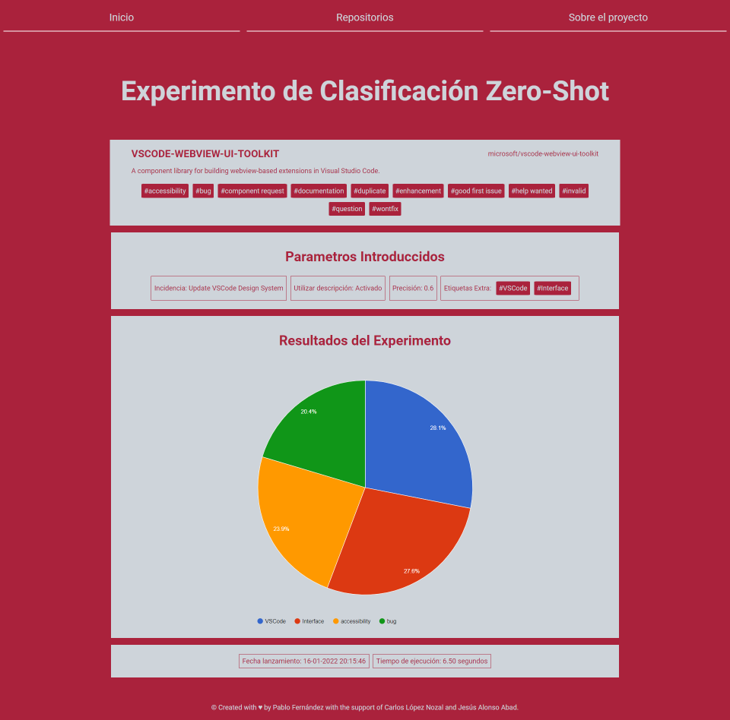
\includegraphics[width=\textwidth]{img/webapp_zsc_output.png}
	\caption{Resultados obtenidos en un experimento de Zero-Shot Classification.}
	\label{fig:webapp_zsc_output}
\end{figure}

\subsubsection{Sentiment Analysis}

Este formulario permite al usuario la aplicación de un modelo de análisis de sentimientos sobre las incidencias del repositorio (véase \autoref{fig:webapp_sa_form}). La finalidad de este experimento radica en la obtención de una puntuación que defina la actitud de los usuarios participantes en la discusión generada por una incidencia. La puntuación obtenida se calcula por cada fragmento y puede variar entre 0 y 1, siendo cero la representación de una expresión de sentimientos muy negativos, y uno la representación de una expresión de sentimientos muy positivos. 

\begin{figure}[!ht]
	\centering
    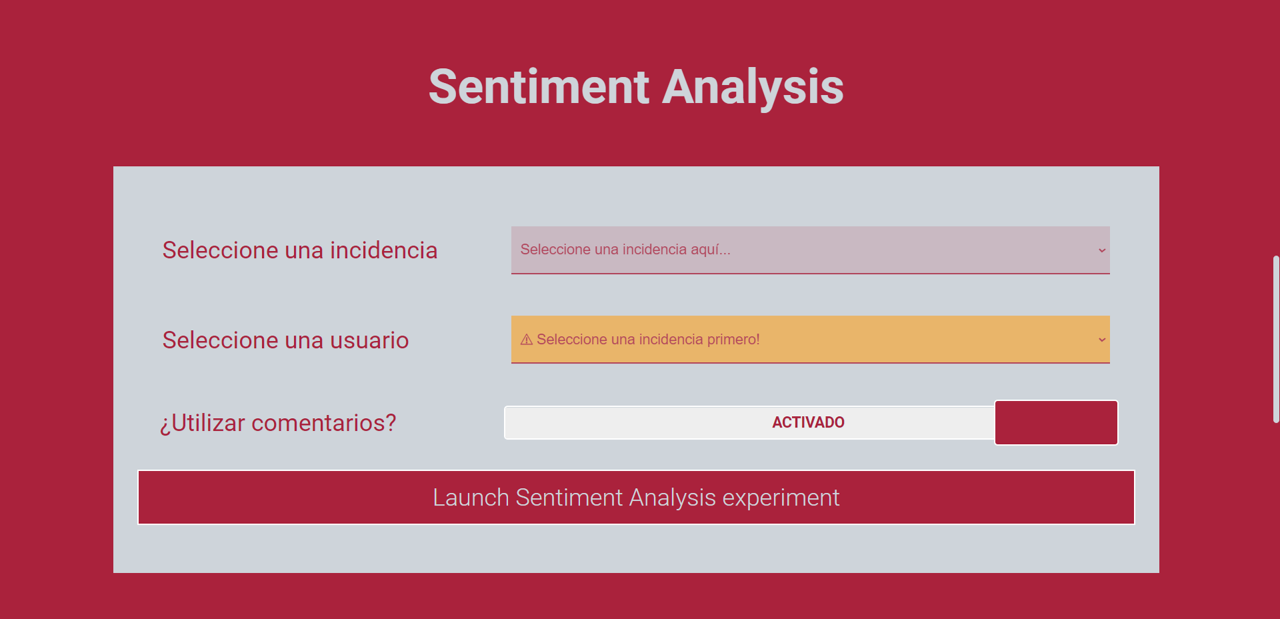
\includegraphics[width=\textwidth]{img/webapp_sa_form.png}
	\caption{Formulario de lanzamiento de experimento de Sentiment Analysis.}
	\label{fig:webapp_sa_form}
\end{figure}

Los parámetros disponibles son los siguientes:

\begin{itemize} \setlength\itemsep{0.2em}
    \item \textbf{Selección de incidencia}. Este parámetro permite seleccionar mediante un desplegable las incidencias del repositorio de acuerdo con su título. 
    \item \textbf{Selección de usuario}. Este parámetro permite filtrar los comentarios de la incidencia que van a ser tomados como entrada del modelo a aquellos realizados exclusivamente por dicho usuario.
    \item Utilizar comentarios. Este parámetro tiene como finalidad permitir la realización del análisis de sentimientos de la entrada inicial de la incidencia, excluyendo sus comentarios tanto del autor como del resto de participantes en la conversación.
\end{itemize}

Los resultados del experimento se presentan haciendo uso de un gráfico de barras verticales. Cada barra azul representa la puntuación otorgada a un comentario, siendo la línea horizontal roja el indicador de la puntuación media obtenida de acuerdo con los parámetros introducidos (véase \autoref{fig:webapp_sa_output}).

\begin{figure}[!ht]
	\centering
    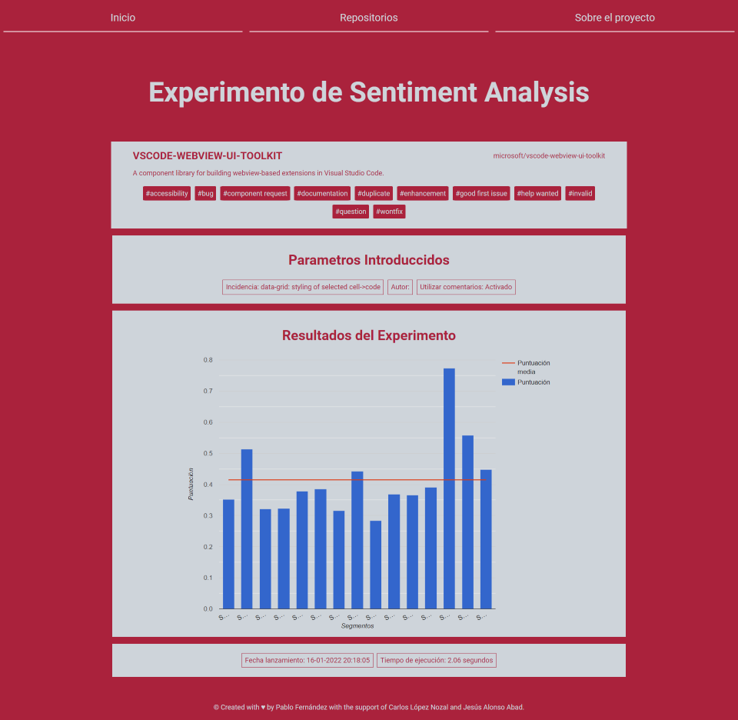
\includegraphics[width=\textwidth]{img/webapp_sa_output.png}
	\caption{Resultados obtenidos en un experimento de Sentiment Analysis.}
	\label{fig:webapp_sa_output}
\end{figure}

\subsubsection{Summarization}

Este formulario permite al usuario el lanzamiento de un experimento de generación de resúmenes abstractivos sobre las incidencias del repositorio (véase \autoref{fig:webapp_summ_form}). La finalidad de este experimento consiste en generar un fragmento de texto que resuma el contenido tratado por la incidencia. El modelo se aplica de manera individual a cada comentario y posteriormente se procede a la concatenación de los resultados para obtener un resumen general del tema tratado en la discusión de la incidencia. Este experimento cuenta con limitaciones lingüísticas debido a que el modelo utilizado que solo ofrece soporte a textos escritos en inglés.

Los parámetros disponibles son los siguientes:

\begin{figure}[!ht]
	\centering
    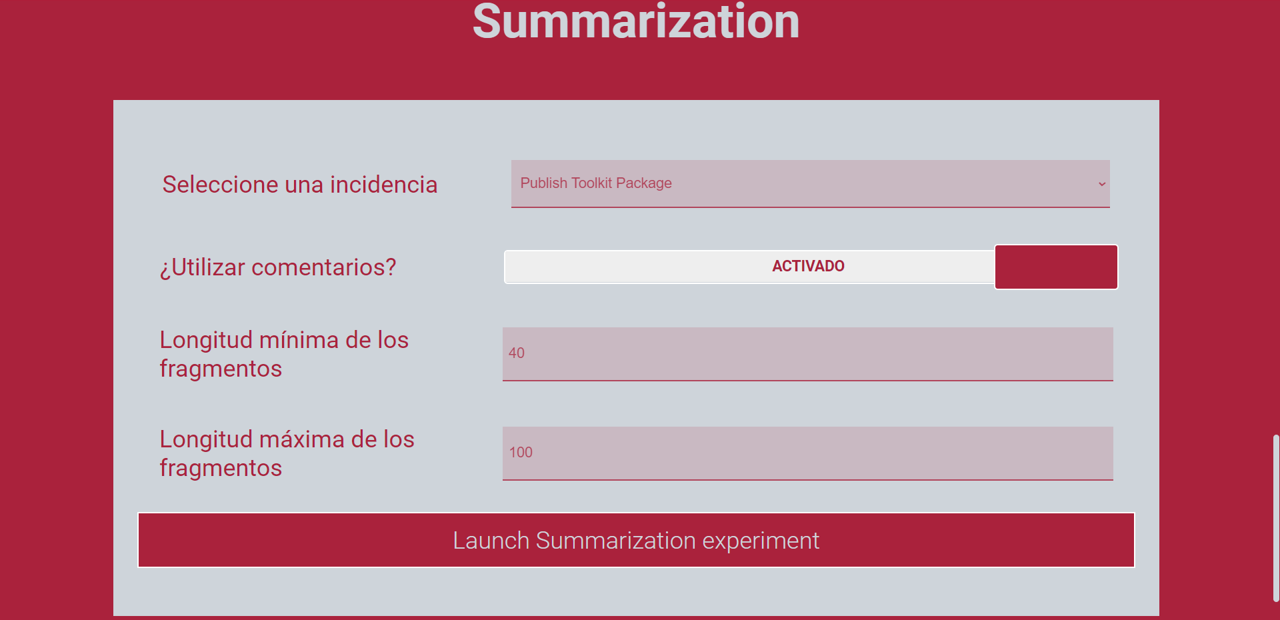
\includegraphics[width=\textwidth]{img/webapp_summ_form.png}
	\caption{Formulario de lanzamiento de experimento de Summarization.}
	\label{fig:webapp_summ_form}
\end{figure}

\begin{itemize} \setlength\itemsep{0.2em}
    \item \textbf{Selección de incidencia}. Este parámetro permite seleccionar mediante un desplegable las incidencias del repositorio de acuerdo con su título.
    \item \textbf{Utilizar descripción}. Este parámetro permite otorgar un mayor contexto al modelo incluyendo la información correspondiente con la descripción de la incidencia en la realización de sus operaciones. Por defecto el modelo sólo utiliza la información deducida a partir de su título.
    \item \textbf{Longitud mínima de los fragmentos}. Este parámetro permite establecer una longitud mínima de los resúmenes parciales que compondrán el resumen final. Es importante destacar el aspecto de los fragmentos, ya que los fragmentos de las entradas se introducen en el modelo de forma individual, por lo tanto el resumen final se elabora a partir de su concatenación. También se ha de destacar que esta longitud no se corresponde directamente con el número de caracteres debido a las consideraciones tomadas por el \textit{tokenizador} utilizado por los modelos.
    \item \textbf{Longitud máxima de los fragmentos}. Este parámetro permite establecer una longitud máxima de los resúmenes parciales que compondrán el resumen final.
\end{itemize}

Los resultados del experimento proveen al usuario del resumen generado en función del contenido de la incidencia y los parámetros de longitud establecidos para cada fragmento (véase \autoref{fig:webapp_summ_output}).

\begin{figure}[!ht]
	\centering
    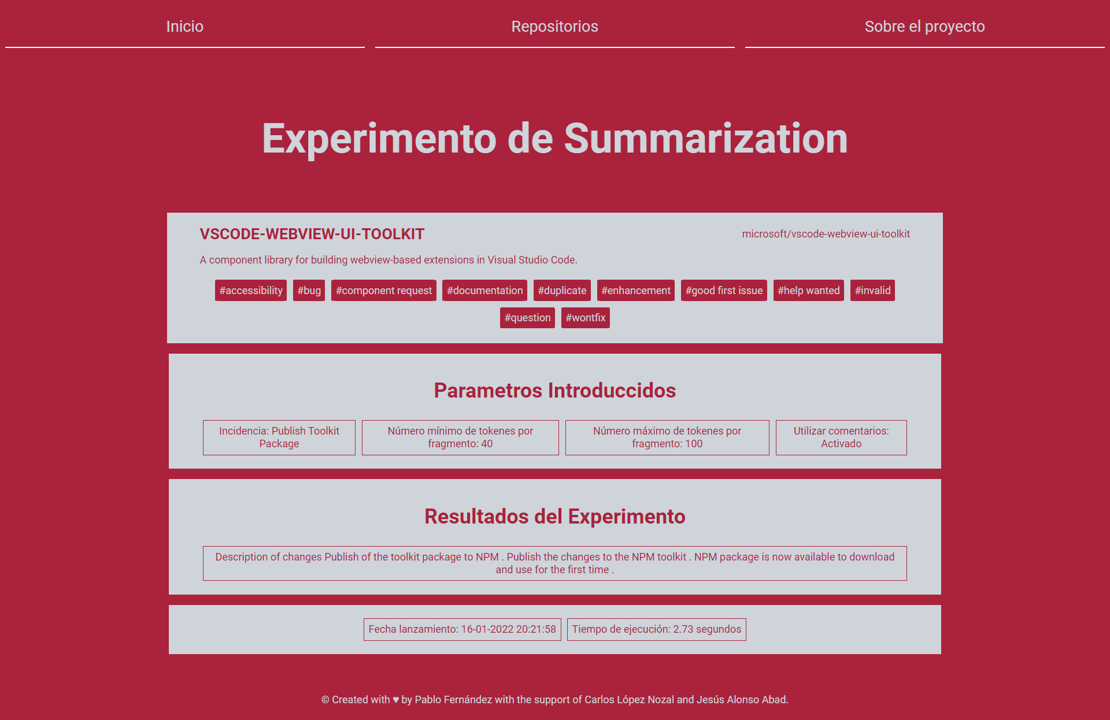
\includegraphics[width=\textwidth]{img/webapp_summ_output.png}
	\caption{Resultados obtenidos en un experimento de Summarization.}
	\label{fig:webapp_summ_output}
\end{figure}